% !TEX root=../../mt-motion-analysis.tex
\chapter{Results and discussion} \label{ch:results}
\section{Body part localization}
om jag f[r tag p[ mer data att validera mot? annars hur?

\section{Classification}
The figures and results presented in this section is generated by models and ensembles trained according to the cross validation strategy described in Section \ref{sec:met-training} and evaluated on the test set. This gives 10 sets of models trained on slightly different data.

\subsection{Trunk}
Figure \ref{fig:trunk-cnf-reps}} shows the confusion matrix summarizing the classifications of the individual repetitions made by the ensemble presented in Table \ref{tab:ensemble-models} and Appendix \ref{}.
Each entry in the matrix is the mean along with the standard deviation for models from the 10 folds. Figures \ref{fig:trunk-cnf-comb}, \ref{fig:trunk-cnf-comb-th} shows the corresponding matrices for the combined scores, with and without the threshold suggested in \ref{sec:met-combined}.
These results are also summarized as accuracy and f1 scores in Table \ref{tab:trunk-results}. This table also shows the model performance performs for the data with different label certainty. Histograms for these metrics are shown in Figure \ref{fig:trunk-hist-results} along with the corresponding metrics for the individual models in the ensemble (high precision models are not shown as they only predict one label).

\begin{table}
  \centering
  \caption{Results of the ensemble for the trunk POE. Rep., Comb., and Thresh. represents the results for the repetitions, combinations, and combinations with thresholds respectively. The Certainties columns shows the results making up the Comb. column, but for the certainty levels of the expert labeling the data. These range from certain (1) to uncertain (3), n shows how many datapoints each category contains. All results are the mean from the 10 folds $\pm$ the corresponding standard deviations.}
  \label{tab:trunk-results}
  \small
  \begin{tabu}[c]{|c|c|c|c||c|c|c|}
    \hline
    % & \multirow21}{*}{Repetitions} & \multirow{2}{*}{Combinations} & \multirow{2}{*}{Thresholds} &  \multirow{2}{*}\multicolumn{3}{c}{Certainties}\\
    & \multirow{2}{*}{\textbf{Rep.}} & \multirow{2}{*}{\textbf{Comb.}} & \multirow{2}{*}{\textbf{Thresh.}} & \multicolumn{3}{c|}{\textbf{Certainties}}\\ \cline{5-7}
    & & & &1(n=15)&2(n=6)&3(n=1)\\ \hline
    Accuracy (\%) &73.7$\pm$4.5&75.0$\pm$7.9&\textbf{80.0$\pm$7.8}&\textbf{81.3$\pm$7.1}&56.7$\pm$15.2&90.0$\pm$30.0\\ \hline
    F1 score (\%) &73.1$\pm$3.4&75.0$\pm$5.8&\textbf{79.9$\pm$8.9}&\textbf{80.4$\pm$7.1}&25.8$\pm$6.3&90.0$\pm$30.0\\ \hline

  \end{tabu}
\end{table}

\begin{figure}
  \centering
  \begin{subfigure}[t]{0.48\textwidth}
      \includegraphics[width=\textwidth]{files/figs/res/trunk/cnf-reps.eps}
      \caption{}
      \label{fig:trunk-cnf-reps}
  \end{subfigure}
  ~
  \begin{subfigure}[t]{0.48\textwidth}
      \includegraphics[width=\textwidth]{files/figs/res/trunk/cnf-combined.eps}
      \caption{}
      \label{fig:trunk-cnf-comb}
  \end{subfigure}

  \begin{subfigure}[t]{0.48\textwidth}
      \includegraphics[width=\textwidth]{files/figs/res/trunk/cnf-combined-th.eps}
      \caption{}
      \label{fig:trunk-cnf-comb-th}
  \end{subfigure}
  \caption{Confusion matrices for the trunk classification on the test set. The entries in the matrices shows the mean and standard deviation of the 10 ensembles trained in the cross validation. Classification of the individual repetitions is shown in (a), the combined score for the sequences of 5 repetitions is shown in (b). (c) shows the combined score with the threshold suggested in Section \ref{sec:met-combined}, i.e. all scores with a predicted probability higher than 0.4.}
  \label{fig:trunk-cnfs}
\end{figure}



\begin{figure}
  \centering
  \begin{subfigure}[t]{0.4\textwidth}
    \includegraphics[width=\textwidth]{files/figs/res/trunk/acc.eps}
    \caption{}
    \label{fig:trunk-acc}
  \end{subfigure}
  ~
  \begin{subfigure}[t]{0.4\textwidth}
    \includegraphics[width=\textwidth]{files/figs/res/trunk/f1.eps}
    \caption{}
    \label{fig:trunk-f1}
  \end{subfigure}

  \begin{subfigure}[t]{0.4\textwidth}
    \includegraphics[width=\textwidth]{files/figs/res/trunk/acc-ind.eps}
    \caption{}
    \label{fig:trunk-acc-ind}
  \end{subfigure}
  ~
  \begin{subfigure}[t]{0.4\textwidth}
    \includegraphics[width=\textwidth]{files/figs/res/trunk/f1-ind.eps}
    \caption{}
    \label{fig:trunk-f1-ind}
  \end{subfigure}
  \caption{Histograms of the accuracies and F1 scores summarized in Table \ref{tab:trunk-results} along with the same metrics for the repetition classification for the models making up the ensembles, presented in Table \ref{tab:ensemble-models}. The high precision models only predicting one class are excluded.}
  \label{fig:trunk-hist-results}
\end{figure}

Based on what is presented in Figures \ref{fig:trunk-cnfs}, \ref{fig:trunk-hist-results} and Table \ref{tab:trunk-results} it seems like the performance of the classifier is enhanced by the measures taken. Table \ref{tab:trunk-improvements} shows this is true with different confidence. Neither the combined score nor the use of an ensemble can be said to improve the performance significantly, but the combined score for the five repetitions is not primarily done to improve the performance, instead this is the way the scoring system is designed. Regarding the ensemble it might be difficult to say how big of an improvement it is based on these metrics, but it reduces the variability in the results. By introducing the threshold, ignoring predictions with a predicted probability lower than 0.4, an average of 3.6 sequences are overlooked. Of these 1.7 were correctly classified and 1.9 were incorrect. %As the compute increases linearly with the number of models used this becomes

From Figure \ref{fig:trunk-cnfs} it is clear that the majority of misclassifications are between the classes 0 and 1. This is a natural effect of there being more 0s and 1s than 2s in the test set. However, asking the experts working with this assessment system these classes are generally the ones difficult to tell apart. Another sign that the model to some extent aligns with the assessments made by the human is the better performance for the sequences where the human expert were certain about the class, seen in Table \ref{tab:trunk-results}.

\begin{table}
  \caption{With what confidence different measures led to improvements. Calculated assuming normal distributions and using pairwise comparisons for the folds. When comparing the ensemble with the individual models the best model is chosen.}
  \label{tab:trunk-improvements}
  \centering
  \begin{tabu}[c]{|c|c|c|c|}
    \hline
    & \multicolumn{1}{c|}{\begin{tabular}[c]{@{}c@{}}\textbf{Ensemble -}\\\textbf{individual} \\\textbf{models}\end{tabular}} &
    \multicolumn{1}{c|}{\begin{tabular}[c]{@{}c@{}}\textbf{Combined -}\\\textbf{Repetitions}\end{tabular}} &
    \multicolumn{1}{c|}{\begin{tabular}[c]{@{}c@{}}\textbf{Threshold -}\\\textbf{Combined}\end{tabular}} \\ \hline
    \textbf{Accuracy} & 85\% & 75\% & 95\% \\ \hline
    \textbf{F1 score} & 75\% & 85\% & 95\% \\ \hline
  \end{tabu}
\end{table}


\begin{figure}
  \centering
  \begin{subfigure}[t]{0.33\textwidth}
    \includegraphics[width=\textwidth]{files/figs/res/trunk/pc0.eps}
    \caption{}
    \label{fig:trunk-pc0}
  \end{subfigure}%
  \begin{subfigure}[t]{0.33\textwidth}
    \includegraphics[width=\textwidth]{files/figs/res/trunk/pc1.eps}
    \caption{}
    \label{fig:trunk-pc1}
  \end{subfigure}%
  \begin{subfigure}[t]{0.33\textwidth}
    \includegraphics[width=\textwidth]{files/figs/res/trunk/pc2.eps}
    \caption{}
    \label{fig:trunk-pc2}
  \end{subfigure}

  \caption{Figures showing the probabilities for the predicted class, without threshold, for correct class 0: (a), 1: (b), 2: (c)}
  \label{fig:trunk-pc}
\end{figure}

In the results above a threshold to ignore uncertain classifications and thereby increase the performance. An extension to such a threshold, and something important for clinical use would be to provide a confidence in the classification. Figure \ref{fig:trunk-pc} shows the probabilities for the predicted class depending on which the correct class actually is. This measure seems to be rather suitable for this, with the model rarely predicting incorrectly when it outputs a high class probability. However, although the ensemble weights has been adjusted as discussed in Section \ref{sec:met-ensembles}, the probabilities for class 1 is generally low.

\FloatBarrier
\subsection{Pelvis}
As for trunk, the pelvis results are presented in Table \ref{tab:pelvis-results}, showing the accuracies and F1 scores and in the confusion matrices in Figure \ref{fig:pelvis-cnfs}. Along with this, histograms showing the effect of the ensemble, combined score, and threshold can be seen in Figure \ref{fig:pelvis-hist-results} and these effects are also summarized in Table \ref{tab:pelvis-improvements}.

Overall it is clear that the performance is worse for the pelvis compared to the other \glspl{poe}. Although the accuracy and F1 score is not that much lower compared to the trunk \gls{poe} it varies much more making it difficult to draw any conclusions from it. It also looks less like a normal distribution, making Table \ref{tab:pelvis-improvements} unreliable. One explanation for this behavior is that the human experts consider this \gls{poe} to be the most difficult one to assess of the four considered in work. The reason for this is that the hip rotates in several planes making it difficult to assess in 2D. This probably affects the models, both directly as a more difficult pattern to identify, which might rely on information not available in this 2D data. It might also affect the models indirectly as this suggests that the training labels can be more unreliable. The threshold neglects 7.6 sequences on average and 4.2 of these were correctly classified. The relatively high number of ignored samples explains higher variance in the accuracy and F1 score.

\begin{table}
  \centering
  \caption{Results of the ensemble for the pelvis POE. Rep., Comb., and Thresh. represents the results for the repetitions, combinations, and combinations with thresholds respectively. The Certainties columns shows the results making up the Comb. column, but for the certainty levels of the expert labeling the data. These range from certain (1) to uncertain (3), n shows how many datapoints each category contains. All results are the mean from the 10 folds $\pm$ the corresponding standard deviations.}
  \label{tab:pelvis-results}
  \small
  \begin{tabu}[c]{|c|c|c|c||c|c|c|}
    \hline
    % & \multirow21}{*}{Repetitions} & \multirow{2}{*}{Combinations} & \multirow{2}{*}{Thresholds} &  \multirow{2}{*}\multicolumn{3}{c}{Certainties}\\
    & \multirow{2}{*}{\textbf{Rep.}} & \multirow{2}{*}{\textbf{Comb.}} & \multirow{2}{*}{\textbf{Thresh.}} & \multicolumn{3}{c|}{\textbf{Certainties}}\\ \cline{5-7}
    & & & &1(n=14)&2(n=7)&3(n=1)\\ \hline
    Accuracy (\%) &63.6$\pm$10.7&69.1$\pm$10.1&\textbf{73.3$\pm$18.9}&67.9$\pm$15.0&\textbf{70.0$\pm$19.6}&80.0$\pm$40.0\\ \hline
    F1 score (\%) &55.7$\pm$13.4&66.5$\pm$15.0&\textbf{73.6$\pm$22.3}&58.0$\pm$20.1&\textbf{63.7$\pm$23.8}&31.7$\pm$17.4\\ \hline
  \end{tabu}
\end{table}


\begin{figure}
  \centering
  \begin{subfigure}[t]{0.48\textwidth}
      \includegraphics[width=\textwidth]{files/figs/res/pelvis/cnf-reps.eps}
      \caption{}
      \label{fig:pelvis-cnf-reps}
  \end{subfigure}
  ~
  \begin{subfigure}[t]{0.48\textwidth}
      \includegraphics[width=\textwidth]{files/figs/res/pelvis/cnf-combined.eps}
      \caption{}
      \label{fig:pelvis-cnf-comb}
  \end{subfigure}

  \begin{subfigure}[t]{0.48\textwidth}
      \includegraphics[width=\textwidth]{files/figs/res/pelvis/cnf-combined-th.eps}
      \caption{}
      \label{fig:pelvis-cnf-comb-th}
  \end{subfigure}
  \caption{Confusion matrices for the pelvis classification on the test set. The entries in the matrices shows the mean and standard deviation of the 10 ensembles trained in the cross validation. Classification of the individual repetitions is shown in (a), the combined score for the sequences of 5 repetitions is shown in (b). (c) shows the combined score with the threshold suggested in Section \ref{sec:met-combined}, i.e. all scores with a predicted probability higher than 0.4.}
  \label{fig:pelvis-cnfs}
\end{figure}

\begin{figure}
  \centering
  \begin{subfigure}[t]{0.4\textwidth}
    \includegraphics[width=\textwidth]{files/figs/res/pelvis/acc.eps}
    \caption{}
    \label{fig:pelvis-acc}
  \end{subfigure}
  ~
  \begin{subfigure}[t]{0.4\textwidth}
    \includegraphics[width=\textwidth]{files/figs/res/pelvis/f1.eps}
    \caption{}
    \label{fig:pelvis-f1}
  \end{subfigure}

  \begin{subfigure}[t]{0.4\textwidth}
    \includegraphics[width=\textwidth]{files/figs/res/pelvis/acc-ind.eps}
    \caption{}
    \label{fig:pelvis-acc-ind}
  \end{subfigure}
  ~
  \begin{subfigure}[t]{0.4\textwidth}
    \includegraphics[width=\textwidth]{files/figs/res/pelvis/f1-ind.eps}
    \caption{}
    \label{fig:pelvis-f1-ind}
  \end{subfigure}
  \caption{Histograms of the accuracies and F1 scores summarized in Table \ref{tab:pelvis-results} along with the same metrics for the repetition classification for the models making up the ensembles, presented in Table \ref{tab:ensemble-models}. The high precision models only predicting one class are excluded.}
  \label{fig:pelvis-hist-results}
\end{figure}

\begin{table}
  \caption{With what confidence different measures led to improvements. Calculated assuming normal distributions and using pairwise comparisons for the folds. When comparing the ensemble with the individual models the best model is chosen.}
  \label{tab:pelvis-improvements}
  \centering
  \begin{tabu}[c]{|c|c|c|c|}
    \hline
    & \multicolumn{1}{c|}{\begin{tabular}[c]{@{}c@{}}\textbf{Ensemble -}\\\textbf{individual} \\\textbf{models}\end{tabular}} &
    \multicolumn{1}{c|}{\begin{tabular}[c]{@{}c@{}}\textbf{Combined -}\\\textbf{Repetitions}\end{tabular}} &
    \multicolumn{1}{c|}{\begin{tabular}[c]{@{}c@{}}\textbf{Threshold -}\\\textbf{Combined}\end{tabular}} \\ \hline
    \textbf{Accuracy} & - & 95\% & 85\% \\ \hline
    \textbf{F1 score} & - & 95\% & 95\% \\ \hline
  \end{tabu}
\end{table}


\begin{figure}
  \centering
  \begin{subfigure}[t]{0.33\textwidth}
    \includegraphics[width=\textwidth]{files/figs/res/pelvis/pc0.eps}
    \caption{}
    \label{fig:pelvis-pc0}
  \end{subfigure}%
  \begin{subfigure}[t]{0.33\textwidth}
    \includegraphics[width=\textwidth]{files/figs/res/pelvis/pc1.eps}
    \caption{}
    \label{fig:pelvis-pc1}
  \end{subfigure}%
  \begin{subfigure}[t]{0.33\textwidth}
    \includegraphics[width=\textwidth]{files/figs/res/pelvis/pc2.eps}
    \caption{}
    \label{fig:pelvis-pc2}
  \end{subfigure}

  \caption{Figures showing the probabilities for the predicted class, without threshold, for correct class 0: (a), 1: (b), 2: (c)}
  \label{fig:pelvis-pc}
\end{figure}


\FloatBarrier
\subsection{Femoral Valgus}
% A confusion matrix showing the mean prediction along with the standard deviation for the 10 ensembles

The results for the femoral valgus \gls{poe} can be found in Figures \ref{fig:femval-cnfs}, \ref{fig:femval-hist-results}, \ref{fig:femval-pc} and Tables \ref{tab:femval-results}, \ref{tab:femval-improvements}.
This model performs a good result, but it seems to be slightly biased, at least for this data, towards class one. On average 2.2 samples are ignored because of the threshold and 1.1 of these were correct. Notable is that it classifies a class 2 as a 0 three times and none of these are ignored due to the threshold. As can be seen in Figure \ref{fig:femval-pc} two of these have a probability right above the threshold of 0.4.

In Table \ref{tab:femval-results} and Figure \ref{fig:femval-hist-results} it can be seeen that the accuracy and F1 score improves by calculating the combined score and by the threshold. For this \gls{poe} the variance is also decreased by introducing the threshold, which was not the case for neither trunk nor pelvis. As can be seen in Table \ref{tab:femval-improvements} the ensemble is not improving the performance, but it gives a more robust model neglecting the poor performance which can be seen for the individual models for one of the folds.

As for the trunk model, the probability for class one is low. This is clearly not a problem for the classification, as mentioned above this model seems to be slightly biased towards class 1. It is however, something to consider for the confidence score desirable in a clinical setting.


LAGG TILL FIGURE MED GRAD CAM!!!!!!

\begin{table}
  \centering
  \caption{Results of the ensemble for the femoral valgus POE. Rep., Comb., and Thresh. represents the results for the repetitions, combinations, and combinations with thresholds respectively. The Certainties columns shows the results making up the Comb. column, but for the certainty levels of the expert labeling the data. These range from certain (1) to uncertain (3), n shows how many datapoints each category contains. All results are the mean from the 10 folds $\pm$ the corresponding standard deviations.}
  \label{tab:femval-results}
  \small
    \begin{tabu}[c]{|c|c|c|c||c|c|c|}
      \hline
      & \multirow{2}{*}{\textbf{Rep.}} & \multirow{2}{*}{\textbf{Comb.}} & \multirow{2}{*}{\textbf{Thresh.}} & \multicolumn{3}{c|}{\textbf{Certainties}}\\ \cline{5-7}
      & & & &1(n=15)&2(n=7)&3(n=0)\\ \hline
      Accuracy (\%) &69.6$\pm$6.8&79.1$\pm$9.3&\textbf{82.3$\pm$6.0}&\textbf{82.7$\pm$9.5}&71.4$\pm$11.0&-\\ \hline
      F1 score (\%) &69.0$\pm$6.6&77.6$\pm$8.6&\textbf{81.0$\pm$5.2}&\textbf{80.8$\pm$8.6}&70.1$\pm$9.4&-\\ \hline

    \end{tabu}
\end{table}

\begin{figure}
  \centering
  \begin{subfigure}[t]{0.48\textwidth}
      \includegraphics[width=\textwidth]{files/figs/res/femval/cnf-reps.eps}
      \caption{}
      \label{fig:femval-cnf-reps}
  \end{subfigure}
  ~
  \begin{subfigure}[t]{0.48\textwidth}
      \includegraphics[width=\textwidth]{files/figs/res/femval/cnf-combined.eps}
      \caption{}
      \label{fig:femval-cnf-comb}
  \end{subfigure}

  \begin{subfigure}[t]{0.48\textwidth}
      \includegraphics[width=\textwidth]{files/figs/res/femval/cnf-combined-th.eps}
      \caption{}
      \label{fig:femval-cnf-comb-th}
  \end{subfigure}
  \caption{Confusion matrices for the femoral valgus classification on the test set. The entries in the matrices shows the mean and standard deviation of the 10 ensembles trained in the cross validation. Classification of the individual repetitions is shown in (a), the combined score for the sequences of 5 repetitions is shown in (b). (c) shows the combined score with the threshold suggested in Section \ref{sec:met-combined}, i.e. all scores with a predicted probability higher than 0.4.}
  \label{fig:femval-cnfs}
\end{figure}





\begin{figure}
  \centering
  \begin{subfigure}[t]{0.4\textwidth}
    \includegraphics[width=\textwidth]{files/figs/res/femval/acc.eps}
    \caption{}
    \label{fig:femval-acc}
  \end{subfigure}
  ~
  \begin{subfigure}[t]{0.4\textwidth}
    \includegraphics[width=\textwidth]{files/figs/res/femval/f1.eps}
    \caption{}
    \label{fig:femval-f1}
  \end{subfigure}

  \begin{subfigure}[t]{0.4\textwidth}
    \includegraphics[width=\textwidth]{files/figs/res/femval/acc-ind.eps}
    \caption{}
    \label{fig:femval-acc-ind}
  \end{subfigure}
  ~
  \begin{subfigure}[t]{0.4\textwidth}
    \includegraphics[width=\textwidth]{files/figs/res/femval/f1-ind.eps}
    \caption{}
    \label{fig:femval-f1-ind}
  \end{subfigure}
  \caption{Histograms of the accuracies and F1 scores summarized in Table \ref{tab:femval-results} along with the same metrics for the repetition classification for the models making up the ensembles, presented in Table \ref{tab:ensemble-models}. The high precision models only predicting one class are excluded.}
  \label{fig:femval-hist-results}
\end{figure}


\begin{table}
  \caption{With what confidence different measures led to improvements. Calculated assuming normal distributions and using pairwise comparisons for the folds. When comparing the ensemble with the individual models the best model is chosen.}
  \label{tab:femval-improvements}
  \centering
  \begin{tabu}[c]{|c|c|c|c|}
    \hline
    & \multicolumn{1}{c|}{\begin{tabular}[c]{@{}c@{}}\textbf{Ensemble -}\\\textbf{individual} \\\textbf{models}\end{tabular}} &
    \multicolumn{1}{c|}{\begin{tabular}[c]{@{}c@{}}\textbf{Combined -}\\\textbf{Repetitions}\end{tabular}} &
    \multicolumn{1}{c|}{\begin{tabular}[c]{@{}c@{}}\textbf{Threshold -}\\\textbf{Combined}\end{tabular}} \\ \hline
    \textbf{Accuracy} & - & 95\% & 95\% \\ \hline
    \textbf{F1 score} & - & 95\% & 95\% \\ \hline
  \end{tabu}
\end{table}


\begin{figure}
  \centering
  \begin{subfigure}[t]{0.33\textwidth}
    \includegraphics[width=\textwidth]{files/figs/res/femval/pc0.eps}
    \caption{}
    \label{fig:femval-pc0}
  \end{subfigure}%
  \begin{subfigure}[t]{0.33\textwidth}
    \includegraphics[width=\textwidth]{files/figs/res/femval/pc1.eps}
    \caption{}
    \label{fig:femval-pc1}
  \end{subfigure}%
  \begin{subfigure}[t]{0.33\textwidth}
    \includegraphics[width=\textwidth]{files/figs/res/femval/pc2.eps}
    \caption{}
    \label{fig:femval-pc2}
  \end{subfigure}

  \caption{Figures showing the probabilities for the predicted class, without threshold, for correct class 0: (a), 1: (b), 2: (c)}
  \label{fig:femval-pc}
\end{figure}




\FloatBarrier
\subsection{Knee Medial-to-Foot Position}
The \gls{kmfp} data is heavily unbalanced making it somewhat difficult to analyze. As long as this training set is a representable class distribution this model might perform satisfactory. However it has seen very few examples of both class 1 and 2, so the risk of out-of-distribution samples if deploying this model is probably rather high. The high variance in the F1 score is explained by the imbalanced data as any misclassification of class 1 or 2 will have a big effect on this.

\begin{figure}
  \centering
  \begin{subfigure}[t]{0.48\textwidth}
      \includegraphics[width=\textwidth]{files/figs/res/kmfp/cnf-reps.eps}
      \caption{}
      \label{fig:kmfp-cnf-reps}
  \end{subfigure}
  ~
  \begin{subfigure}[t]{0.48\textwidth}
      \includegraphics[width=\textwidth]{files/figs/res/kmfp/cnf-combined.eps}
      \caption{}
      \label{fig:kmfp-cnf-comb}
  \end{subfigure}

  \begin{subfigure}[t]{0.48\textwidth}
      \includegraphics[width=\textwidth]{files/figs/res/kmfp/cnf-combined-th.eps}
      \caption{}
      \label{fig:kmfp-cnf-comb-th}
  \end{subfigure}
  \caption{Confusion matrices for the KMFP classification on the test set. The entries in the matrices shows the mean and standard deviation of the 10 ensembles trained in the cross validation. Classification of the individual repetitions is shown in (a), the combined score for the sequences of 5 repetitions is shown in (b). (c) shows the combined score with the threshold suggested in Section \ref{sec:met-combined}, i.e. all scores with a predicted probability higher than 0.4.}
  \label{fig:kmfp-cnfs}
\end{figure}

\begin{table}
  \centering
  \caption{Results of the ensemble for the KMFP POE. Rep., Comb., and Thresh. represents the results for the repetitions, combinations, and combinations with thresholds respectively. The Certainties columns shows the results making up the Comb. column, but for the certainty levels of the expert labeling the data. These range from certain (1) to uncertain (3), n shows how many datapoints each category contains. All results are the mean from the 10 folds $\pm$ the corresponding standard deviations.}
  \label{tab:kmfp-results}
  \small
    \begin{tabu}[c]{|c|c|c|c||c|c|c|}
      \hline
      % & \multirow21}{*}{Repetitions} & \multirow{2}{*}{Combinations} & \multirow{2}{*}{Thresholds} &  \multirow{2}{*}\multicolumn{3}{c}{Certainties}\\
      & \multirow{2}{*}{\textbf{Rep.}} & \multirow{2}{*}{\textbf{Comb.}} & \multirow{2}{*}{\textbf{Thresh.}} & \multicolumn{3}{c|}{\textbf{Certainties}}\\ \cline{5-7}
      & & & &1(n=19)&2(n=2)&3(n=1)\\ \hline
      Accuracy (\%) &82.3$\pm$3.1&89.5$\pm$4.5&\textbf{90.3$\pm$4.3}&\textbf{92.6$\pm$5.3}&90.0$\pm$20.0&30.0$\pm$45.8\\ \hline
      F1 score (\%) &65.1$\pm$13.7&69.0$\pm$24.6&\textbf{74.0$\pm$22.3}&\textbf{69.3$\pm$28.6}&57.8$\pm$17.8&10.0$\pm$15.3\\ \hline

    \end{tabu}
\end{table}


\begin{figure}
  \centering
  \begin{subfigure}[t]{0.4\textwidth}
    \includegraphics[width=\textwidth]{files/figs/res/kmfp/acc.eps}
    \caption{}
    \label{fig:kmfp-acc}
  \end{subfigure}
  ~
  \begin{subfigure}[t]{0.4\textwidth}
    \includegraphics[width=\textwidth]{files/figs/res/kmfp/f1.eps}
    \caption{}
    \label{fig:kmfp-f1}
  \end{subfigure}

  \begin{subfigure}[t]{0.4\textwidth}
    \includegraphics[width=\textwidth]{files/figs/res/kmfp/acc-ind.eps}
    \caption{}
    \label{fig:kmfp-acc-ind}
  \end{subfigure}
  ~
  \begin{subfigure}[t]{0.4\textwidth}
    \includegraphics[width=\textwidth]{files/figs/res/kmfp/f1-ind.eps}
    \caption{}
    \label{fig:kmfp-f1-ind}
  \end{subfigure}
  \caption{Histograms of the accuracies and F1 scores summarized in Table \ref{tab:kmfp-results} along with the same metrics for the repetition classification for the models making up the ensembles, presented in Table \ref{tab:ensemble-models}. The high precision models only predicting one class are excluded.}
  \label{fig:kmfp-hist-results}
\end{figure}


\begin{table}
  \caption{With what confidence different measures led to improvements. Calculated assuming normal distributions and using pairwise comparisons for the folds. When comparing the ensemble with the individual models the best model is chosen.}
  \label{tab:kmfp-improvements}
  \centering
  \begin{tabu}[c]{|c|c|c|c|}
    \hline
    & \multicolumn{1}{c|}{\begin{tabular}[c]{@{}c@{}}\textbf{Ensemble -}\\\textbf{individual} \\\textbf{models}\end{tabular}} &
    \multicolumn{1}{c|}{\begin{tabular}[c]{@{}c@{}}\textbf{Combined -}\\\textbf{Repetitions}\end{tabular}} &
    \multicolumn{1}{c|}{\begin{tabular}[c]{@{}c@{}}\textbf{Threshold -}\\\textbf{Combined}\end{tabular}} \\ \hline
    \textbf{Accuracy} & - & 95\% & 95\% \\ \hline
    \textbf{F1 score} & - & 95\% & 95\% \\ \hline
  \end{tabu}
\end{table}


\begin{figure}
  \centering
  \begin{subfigure}[t]{0.33\textwidth}
    \includegraphics[width=\textwidth]{files/figs/res/kmfp/pc0.eps}
    \caption{}
    \label{fig:kmfp-pc0}
  \end{subfigure}%
  \begin{subfigure}[t]{0.33\textwidth}
    \includegraphics[width=\textwidth]{files/figs/res/kmfp/pc1.eps}
    \caption{}
    \label{fig:kmfp-pc1}
  \end{subfigure}%
  \begin{subfigure}[t]{0.33\textwidth}
    \includegraphics[width=\textwidth]{files/figs/res/kmfp/pc2.eps}
    \caption{}
    \label{fig:kmfp-pc2}
  \end{subfigure}

  \caption{Figures showing the probabilities for the predicted class, without threshold, for correct class 0: (a), 1: (b), 2: (c)}
  \label{fig:kmfp-pc}
\end{figure}

\subsection{Summary}
Should the results of the classification be summarized it can be said that the model for femoral valgus seems to perform the best followed by pelvis. \gls{kmfp} probably performs satisfactory on this data, but the class imbalance makes it difficult to assess. The pelvis model does not perform very well which might be due to that it is based on information not available in the 2D joint position data, or that more data and different models are needed.

kanske summera accuracies osv har ocks[..
